\documentclass[journal=tches,spthm]{iacrtrans}
\usepackage[T1]{fontenc}
\usepackage[T1]{fontenc}
\usepackage[utf8]{inputenc}
\usepackage{makecell}
\usepackage{todonotes}
\usepackage{subfigure}
\usepackage{amsmath,amssymb,amsfonts}
\usepackage{mathtools}
\usepackage{arydshln}
\usepackage{underscore}
\usepackage{hyperref} % before url package otherwise there is a pb
\hypersetup{
   pdftitle={EdMSM: Multi-Scalar-Multiplication for recursive SNARKs and more},    %title
   pdfauthor={Gautam Botrel and Youssef El Housni},            % author
   pdfsubject={Cryptography},           % subject of the document
   pdfkeywords={},%
   colorlinks=true,         % false: boxed links; true: colored links
   linkcolor=black,         % color of internal links
   citecolor=black,         % color of links to bibliography
   filecolor=black,         % color of file links
   urlcolor=black,          % color of external links
}
\usepackage{pgf}
\usepackage{pifont}
\newcommand{\ymark}{\ding{51}}%
\newcommand{\nmark}{\ding{55}}%
\newcommand{\MGray}{gray}
\newcommand{\MBlue}{blue}
\newcommand{\MOrange}{orange}
\newcommand{\MBlueII}{teal}
\newcommand{\MNavyBlue}{blue!70!black}
\newcommand{\MRed}{red}
\newcommand{\MRedII}{red!60!black}
\newcommand{\MGreen}{green!80!black}
\newcommand{\red}[1]{\textcolor{red}{#1}}
\newcommand{\blue}[1]{\textcolor{blue}{#1}}
\usepackage{pgfplots}
\usepackage{pgfmath,pgffor}

\usepackage{tikz}
 \newcommand\Bucket[1]{%
   \tikz[baseline=(char.base)]\node[rectangle,draw,inner sep=2pt] (char) {#1};}

\usetikzlibrary{arrows,automata}
\usetikzlibrary{positioning}
\tikzset{
  state/.style={
    rectangle,
    rounded corners,
    draw=black, thick,
    minimum height=2em,
    inner sep=2pt,
    text centered,
  },
}
\usetikzlibrary{tikzmark}
\usepackage{url}
\usepackage[onelanguage,tworuled,noline,noend,linesnumbered]{algorithm2e}

\title{EdMSM: Multi-Scalar-Multiplication for recursive SNARKs and more}

\author{Gautam Botrel \inst{1} \and Youssef El Housni \inst{1,2,3}}
\institute{ConsenSys R\&D, gnark team  \\
   \email{{firstname.lastname}@consensys.net}
  \and
    LIX, CNRS, \'{E}cole Polytechnique, Institut Polytechnique de Paris
  \and
    Inria
}

\date{\today}
\newcommand{\MLightBlue}{blue!25!white}
\newcommand{\bfm}{{\bf m}}
\newcommand{\bfa}{{\bf a}}
\newcommand{\bfs}{{\bf s}}
\newcommand{\bff}{{\bf f}}
\newcommand{\bfc}{\text{Cost}}
\newcommand{\bfi}{{\bf i}}
\newcommand{\N}{\ensuremath{\mathbb N}}
\newcommand{\Z}{\ensuremath{\mathbb Z}}
\newcommand{\Q}{\ensuremath{\mathbb{Q}}}
\newcommand{\C}{\ensuremath{\texttt{C}}}
\newcommand{\F}{\ensuremath{\mathbb F}}
\newcommand{\G}{\ensuremath{\mathbb G}}
\newcommand{\T}{\ensuremath{\mathbb{T}}}
\newcommand{\Fp}{\F_p}
\newcommand{\cO}{\ensuremath{\mathcal O}}
\DeclareMathOperator{\Div}{div}
\DeclareMathOperator{\GF}{GF}
\DeclareMathOperator{\Tate}{Tate}
\DeclareMathOperator{\ate}{ate}
\DeclareMathOperator{\End}{End}
\newcommand{\BN}{\ensuremath{\mathrm{BN}}}
\newcommand{\bn}{\ensuremath{\mathrm{bn}}}
\newcommand{\BLS}{\ensuremath{\mathrm{BLS}}}
\newcommand{\BW}{\ensuremath{\mathrm{BW}}}
\newcommand{\bw}{\ensuremath{\mathrm{bw}}}
\newcommand{\CP}{\ensuremath{\mathrm{CP}}}
\newcommand{\cp}{\ensuremath{\mathrm{cp}}}
\newcommand{\bls}{\ensuremath{\mathrm{bls}}}

\begin{document}
\maketitle

\keywords{elliptic curves \and multi-scalar-multiplication \and implementation \and zero-knowledge proof}

\begin{abstract}
The bottleneck in the proving algorithm of most of elliptic-curve-based SNARK
    proof systems is the Multi-Scalar-Multiplication (MSM) algorithm. In this
    paper we give an overview of a variant of the Pippenger MSM algorithm
    together with a set of optimizations tailored for curves that admit a
    twisted Edwards form. This is the case for SNARK-friendly chains and cycles
    of elliptic curves, which are useful for recursive constructions.

Accelerating the MSM over these curves on mobile devices is critical
    for deployment of recursive proof systems on mobile applications.
    This work is implemented in Go and uses hand-written
    \texttt{arm64} assembly for accelerating the finite field
    arithmetic (\texttt{bigint}).  This work was implemented as part
    of a submission to the ZPrize competition in the open division
    ``Accelerating MSM on Mobile'' (\url{https://www.zprize.io/}).
    We achieved a 78\% speedup over the ZPrize baseline implementation
    in Rust.
\end{abstract}

\section{Introduction}
A SNARK is a cryptographic primitive that enables a prover to prove to a
verifier the knowledge of a satisfying witness to a non-deterministic (NP)
statement by producing a proof $\pi$ such that the size of $\pi$ and the cost
to verify it are both sub-linear in the size of the witness. Today, the most
efficient SNARKs use elliptic curves to generate and verify the proof.  A SNARK
usually consists in three algorithms \textit{Setup}, \textit{Prove} and
\textit{Verify}.

The \textit{Setup} and \textit{Prove} algorithms involve solving multiple large
instances of tasks about polynomial arithmetic in $\F_r[X]$ and multi-scalar
multiplication (MSM) over the points of an elliptic curve.  Fast arithmetic in
$\F_r[X]$, when manipulating large-degree polynomials, is best implemented
using the Fast Fourier Transform (FFT)~\cite{jMoC:Pollard71} and MSMs of large
sizes are best implemented using a variant of Pippenger's
algorithm~\cite[Section~4]{INDOCRYPT:BDLO12}. For example,
Table~\ref{tab:g16-plonk-cost} reports the numbers of MSMs required in the
\textit{Setup}, \textit{Prove} and \textit{Verify} algorithms in
the~\cite{EC:Groth16} SNARK and the KZG-based PLONK universal
SNARK~\cite{EPRINT:GabWilCio19}. The report excludes the number of FFTs as the
dominating cost for such constructions is the MSM computation ($\sim 80\%$ of the overall time).
%
\begin{table}[htb]
  \caption{Cost of \texttt{Setup}, \texttt{Prove} and \texttt{Verify}
      algorithms for~\cite{EC:Groth16} and PLONK. $m=$ number of wires, $n=$ number of
      multiplication gates, $a=$ number of addition gates and $\ell=$ number of
      public inputs. \texttt{M}$_{\G}=$ multiplication in $\G$ and
      \texttt{P}=pairing. \textit{Note:} Both Groth16 and PLONK verifiers have a dependency on
      the number of public inputs $\ell$, but for PLONK it is just a polynomial
      evaluation (FFT).}
  \label{tab:g16-plonk-cost}
  \centering
  $\begin{array}{|l|c|c|c|}
    \hline
              & \texttt{Setup} & \texttt{Prove} & \texttt{Verify}  \\
    \hline
      \text{\cite{EC:Groth16}} & \makecell{3n \texttt{ M}_{\G_1} \\ m \texttt{ M}_{\G_2}} & \makecell{(3n+m-\ell) \texttt{ M}_{\G_1} \\ n \texttt{ M}_{\G_2} } & \makecell{3 \texttt{ P} \\ \ell \texttt{ M}_{\G_1}}  \\
    \hline
      \text{PLONK (KZG)}   & \makecell{d~{(\geq n+a)} \texttt{ M}_{\G_1} \\ 1 \texttt{ M}_{\G_2} } & 9(n+a) \texttt{ M}_{\G_1} & \makecell{2 \texttt{ P} \\ 18 \texttt{ M}_{\G_1}} \\
    \hline
  \end{array}$
\end{table}

Given a set of $n$ elements $G_1, \cdots, G_n$ (bases) in $\G$ a cyclic group (e.g.~group of points on an elliptic curve)
whose order $\#\G$ has $b$-bit and a set of $n$ integers $a_1, \cdots, a_n$
(scalars) between $0$ and $\#\G$, the goal is to compute efficiently the group
element $[a_1]G_1 + \cdots + [a_n]G_n$. In SNARK applications, we are
interested in large instances of variable-base MSMs ($n=10^7,10^8,10^9$) — with random
bases and random scalars — over the pairing groups $\G_1$ and $\G_2$.

The naive algorithm uses a double-and-add strategy to compute each $[a_i]G_i$
then adds them all up, costing on average $3/2 \cdot b \cdot n$ group
operations ($+$). There are several algorithms that optimize the total number
of group operations as a function of $n$ such as Strauss~\cite{amm:Strauss64},
Bos--Coster~\cite[Sec.~4]{EC:deRooij94} and Pippenger~\cite{focs:Pippenger76}
algorithms. For large instances of a variable-base MSM, the fastest approach is
a variant of Pippenger's algorithm~\cite[Sec.~4]{INDOCRYPT:BDLO12}. For
simplicity, we call it the bucket method. In this paper we are interested
in the bucket-method MSM on inner curves of 2-chains and 2-cycles of elliptic
curves.  We've chosen to test and benchmark our results on mobile devices
because it is critical for deployment of recursive proof systems on mobile
applications.
%
\paragraph{Organization of the paper.}
Section~\ref{sec:2-chain-cycle} provides definitions of 2-chains and 2-cycles
of elliptic curves and some results we prove.  In section~\ref{sec:bucket-msm},
we explain the bucket method and provide its complexity analysis.  The core of
the paper are sections~\ref{sec:optimizations} and~\ref{sec:implementation}.
Section~\ref{sec:optimizations} provides our optimizations to the bucket method
for both generic elliptic curves and the twisted Edwards curves. We prove that
inner 2-chains and 2-cycles always fall into the second more optimized case.
Finally, section~\ref{sec:implementation} reports on our implementation of the
bucket method alongside our optimizations. We choose to tailor the
implementation to the widely used BLS12-377 curve and to benchmark our results
on a mobile widely available mobile device.
%
\section{2-chain and 2-cycle of elliptic curves}
\label{sec:2-chain-cycle}
\subsection{2-chains}
\label{2-chains}
Following~\cite{EC:HouGui22}, a 2-chain of elliptic curves is a
set of two curves as in Definition~\ref{def:m-chain-snark-friendly}.
%
\begin{definition}
  A $2$-chain of elliptic curves is a list of two distinct curves
    $E_1/\F_{p_1}$ and $E_1/\F_{p_2}$ where $p_1$ and $p_2$ are large primes
    and $p_1 \mid \# E_2(\F_{p_2})$.  SNARK-friendly 2-chains are composed of
    two curves that have highly 2-adic subgroups of orders $r_1 \mid \#
    E_1(\F_{p_1})$ and $r_2 \mid \# E_2(\F_{p_2})$ such that~$r_1 \equiv r_2
    \equiv 1 \mod 2^L$ for a large integer $L \geq 1$. This also means that
    $p_1 \equiv 1 \mod 2^L$.
    \label{def:m-chain-snark-friendly}
\end{definition}
%
In a 2-chain, the first curve is denoted the \textit{inner curve}, while the
second curve whose order is the characteristic of the inner curve, is denoted
the \textit{outer curve} (cf.~Fig.~\ref{figure:EC-chain}).
%
\begin{figure}[htb]
  \centering
  {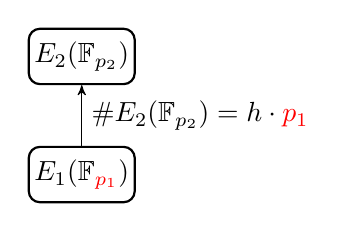
\begin{tikzpicture}[->,>=stealth']
      \node[state] (E2)
    {
      \textbf{$E_2(\F_{p_2})$}
    };
    \node[state, below of=E2, node distance=1.5cm] (E1)
    {
        \textbf{$E_1(\F_{\textcolor{red}{p_1}})$}
    };
      \path (E1) edge node[anchor=west]{$\#E_2(\F_{p_2}) = h \cdot \textcolor{red}{p_1}$} (E2);
  \end{tikzpicture}}
\caption{A 2-chain of elliptic curves.}
  \label{figure:EC-chain}
\end{figure}
%
\paragraph{Inner curves from polynomial families.}
The best elliptic curves amenable to efficient
implementations arise from polynomial based families. These curves are obtained
by parameterizing the Complex Multiplication (CM) equation with polynomials $p(x), t(x), r(x)$ and
$y(x)$.  The authors of~\cite{EC:HouGui22} showed that the polynomial-based
pairing-friendly Barreto--Lynn--Scott families of embedding degrees $k=12$
(BLS12) and $k=24$ (BLS24)~\cite{SCN:BarLynSco02} are the most
suitable to construct inner curves in the context of pairing-based SNARKs. These curves
require the seed $x$ to satisfy $x \equiv 1 \bmod 3\cdot 2^{L}$
to have the 2-adicity requirement with respect to both $r$ and $p$.

A particular example of an efficient 2-chain for SNARK applications is composed
of the inner curve BLS12-377~\cite{SP:BCGMMW20} and the outer curve
BW6-761~\cite{CANS:HouGui20}.

We prove useful results (Prop.~\ref{prop:b=1} and
Lemma~\ref{lemma:msm-inner-bls}) that will be needed later to optimize the MSM
computation.
%
\begin{proposition}[{\cite[Sec.~3.4]{EC:HouGui22}}]
\label{prop:b=1}
    All inner BLS curves admit a short Weierstrass form $Y^2=X^3+1$.
\end{proposition}

\begin{proof}
    Let $E:Y^2=X^3+b$ be a BLS curve over $\F_p$ parametrized by polynomials in
    $x$~\cite{SCN:BarLynSco02}. Let $g$ neither a square nor a cube in $\F_p$.
    One choice of $b \in \{1,g,g^2,g^3,g^4,g^5\}$ gives a curve with the
    correct order (i.e. $r \mid \#E(\F_p)$)~\cite[\S{}X.5]{Silverman09}. For
    all BLS curves, $x-1 \mid \#E(\F_p)$ and $3 \mid x-1$ (which leads to all
    involved parameters being integers)~\cite{SCN:BarLynSco02}. If,
    additionally, $2 \mid x-1$ then $2,3\mid \#E(\F_p)$ and the curve has
    points of order 2 and 3.  A 2-torsion point is $(x_0,0)$ with $x_0$ a root
    of $x^3 + b$, hence $b=(-x_0)^3$ is a cube.  The two 3-torsion points are
    $(0,\pm \sqrt{b})$ hence $b$ is a square.  This implies that $b$ is a
    square and a cube in $\F_p$ and therefore $b=1$ is the only solution in the
    set $\{g^i\}_{0\leq i \leq 5}$ for half of all BLS curves: those with odd
    $x$.

    An inner BLS curve has a seed $x$ such that $x \equiv 1 \mod 3\cdot 2^L$
    for some large integer $L$~\cite{EC:HouGui22}. This means that $2 \mid
    x-1$ and hence that the curve is always of the form $Y^2=X^3+1$.
\end{proof}

\begin{lemma}
    \label{lemma:msm-inner-bls}
    All inner BLS curves admit a twisted
    Edwards form $ay^2+x^2=1+dx^2y^2$ with $a=2\sqrt{3}-3$ and $d=-2\sqrt{3}-3$
    over $\F_p$. If further $-a$ is a square, the equation becomes
    $-x^2+y^2=1+d'x^2y^2$ with $d'=7+4\sqrt{3} \in \F_p$.
\end{lemma}

\begin{proof}
    Proposition~\ref{prop:b=1} shows that all inner BLS curves are of the form
    $W_{0,1}:\, y^2=x^3+1$. The following map
    \begin{align*}
        W_{0,1} &\rightarrow E_{a,d} \\
        (x,y) &\mapsto (\frac{x+1}{y}, \frac{x+1-\sqrt{3}}{x+1+\sqrt{3}})
    \end{align*}
    defines the curve $E_{a,d}:\, ay^2+x^2=1+dx^2y^2$ with $a=2\sqrt{3}-3$ and $d=-2\sqrt{3}-3$.
    The inverse map is
    \begin{align*}
        E_{a,d} &\rightarrow W_{0,1} \\
        (x,y) &\mapsto (\frac{(1+y)\sqrt{3}}{1-y}-1, \frac{(1+y)\sqrt{3}}{(1-y)x})
    \end{align*}

    If $-a$ is a square in $\F_p$, the map $(x,y) \mapsto (x/\sqrt{-a}, y)$
    defines from $E_{a,d}$ the curve $E_{-1,d'}$ of equation
    $-x^2+y^2=1+d'x^2y^2$ with $d'=-d/a=(2\sqrt{3}+3)/(2\sqrt{3}-3)=7+4\sqrt{3}$.

    These maps work only if $\sqrt{3}$ is defined in $\F_p$, that is $3$ is a
    quadratic residue. This is always the case in $\F_p$ on which an inner BLS
    curve is defined. Let $\left(\dfrac{3}{p}\right)$ be $3^{\frac{p-1}{2}}
    \mod p$, the Legendre symbol. The quadratic reciprocity theorem tells us that
    $\left(\dfrac{3}{p}\right)\left(\dfrac{p}{3}\right)=(-1)^{\frac{p-1}{2}}$.
    We have $p \equiv 1 \mod 4$ from the 2-adicity condition, so
    $\left(\dfrac{3}{p}\right)=\left(\dfrac{p}{3}\right)$.  Now
    $\left(\dfrac{p}{3}\right) \equiv p \mod 3$ which is always equal to $1$
    for all BLS curves ($x \equiv 1 \mod 3$ and $x-1 \mid p-1$). More
    generally one can prove that when $p=2$ or $p \equiv 1$ or $11 \mod 12$
    then 3 is a quadratic residue in $\F_p$. For inner BLS, we have $p \equiv 1
    \mod 3\cdot 2^L$ with $L \gg 2$.
\end{proof}

\subsection{2-cycles}
\begin{definition}
  A $2$-cycle of elliptic curves is a list of two distinct prime-order curves
    $E_1/\F_{p_1}$ and $E_1/\F_{p_2}$ where $p_1$ and $p_2$ are large primes,
    $p_1 = \# E_2(\F_{p_2})$ and $p_2 = \# E_1(\F_{p_1})$. SNARK-friendly
    2-cycles are composed of two curves that have highly 2-adic subgroups,
    i.e.~$\# E_1(\F_{p_1}) \equiv \# E_2(\F_{p_2})  \equiv 1 \mod 2^L$ for a
    large integer $L \geq 1$. This also means that $p_1 \equiv p_2 \equiv 1
    \mod 2^L$.
    \label{def:m-chain-snark-friendly}
\end{definition}
%
This notion was initially introduced under different names, for example
\emph{amicable pairs} (or equivalently \emph{dual elliptic
primes}~\cite{EPRINT:Mihailescu07}) for 2-cycles of ordinary curves,
and~\emph{aliquot cycles} for the general case~\cite{EM:SilSta11}. Some
examples of SNARK-friendly 2-cycles include MNT4-MNT6 curves~\cite{C:BCTV14},
Tweedle curves~\cite{EPRINT:BowGriHop19} and Pasta
curves~\cite{post:Hopwood21}.

In particular a 2-cycle is a 2-chain where both curves are inner and outer
curves with respect to each other (cf.~Fig.~\ref{figure:EC-cycle}). This means
that both curves in a 2-cycle admit a twisted Edwards form following the same
reasoning as in subsection~\ref{2-chains}. In the sequel we will focus on the
case of BLS12 inner curves that form a 2-chain but we stress that these results
apply to 2-chain inner curves from other families (e.g.~BLS24 and
BN~\cite{EPRINT:AraHouGui22}) and to 2-cycles as well.
%
\begin{figure}[htb]
  \centering
  {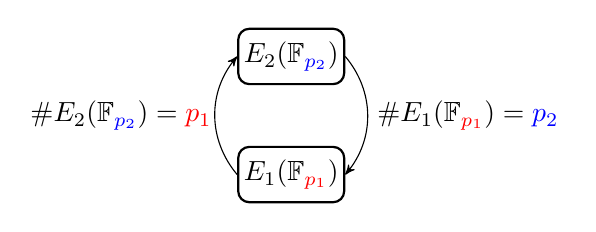
\begin{tikzpicture}[->,>=stealth']
      \node[state] (E2)
    {
        \textbf{$E_2(\F_{\textcolor{blue}{p_2}})$}
    };
    \node[state, below of=E2, node distance=1.5cm] (E1)
    {
      \textbf{$E_1(\F_{\textcolor{red}{p_1}})$}
    };

      \path (E2.east) edge[bend left=40] node[anchor=west]{$\#E_1(\F_{\textcolor{red}{p_1}}) = \textcolor{blue}{p_2}$} (E1.east);
      \path (E1.west) edge[bend left=40] node[anchor=east,inner sep=1.0pt]{$\#E_2(\F_{\textcolor{blue}{p_2}}) = \textcolor{red}{p_1}$} (E2.west);
  \end{tikzpicture}}
\caption{A cycle of elliptic curves.}
  \label{figure:EC-cycle}
\end{figure}
%
\section{The bucket method}
\label{sec:bucket-msm}
The high-level strategy of the bucket-method MSM can be given in three steps:
\begin{itemize}
\item Step 1: reduce the $b$-bit MSM to several $c$-bit MSMs for some fixed $c \leq b$
\item Step 2: solve each $c$-bit MSM efficiently
\item Step 3: combine the $c$-bit MSMs into the final $b$-bit MSM
\end{itemize}

\subsection{Step 1: reduce the $b$-bit MSM to several $c$-bit MSMs}
\begin{enumerate}
\item Choose a window $c \leq b$
\item Write each scalar $a_1, \cdots, a_n$ in binary form and partition each into $c$-bit parts
    $$ a_i = (\underbrace{a_{i,1}, a_{i,2}, \cdots, \underbrace{a_{i,b/c}}_\text{$c$-bit}}_\text{$b$-bit})_{2} $$
\item Deduce $b/c$ instances of $c$-bit MSMs from the partitioned scalars
    \begin{align*}
        T_1 &= [a_{1,1}]G_1 + \cdots + [a_{n,1}]G_n \\
        &\vdots \\
        T_j &= [a_{1,j}]G_1 + \cdots + [a_{n,j}]G_n \\
        &\vdots \\
        T_{b/c} &= [a_{1,b/c}]G_1 + \cdots + [a_{n,b/c}]G_n
    \end{align*}
\end{enumerate}

\begin{center}
    \framebox[1.1\width]{Cost of Step 1 is negligible.}
\end{center}

\subsection{Step 3: combine the $c$-bit MSMs into the final $b$-bit MSM\\}
Algorithm~\ref{alg:msm-step3} gives an iterative way to combine the small MSMs into the original MSM.
%
\begin{algorithm}[hbt]
  \SetAlgoLined
  \KwOut{$T = [a_1]G_1 + \cdots + [a_n]G_n$}
   $T \leftarrow T_1$\;
   \For{$i$ from $2$ to $b/c$}{
     $T \gets [2^c]T$\tcp*[r]{\textsc{Double $c$ times}}
     $T \gets T+T_i$\tcp*[r]{\textsc{Add}}
   }
  \Return $T$\;
  \caption{Step 3}
  \label{alg:msm-step3}
\end{algorithm}

\begin{center}
    \framebox[1.1\width]{Cost of Step 3: $(b/c-1)(c+1) = b-c+b/c-1$ group operations.}
\end{center}

\subsection{Step 2: solve each $c$-bit MSM $T_j$ efficiently}
\begin{enumerate}
    \item For each $T_j$, accumulate the bases $G_i$ inside buckets \\
        Each element $a_{i,j}$ is in the set $\{0,1,2, \cdots 2^c-1\}$. We initialize $2^c-1$ empty buckets (with points at infinity) and accumulate the bases $G_i$ from each $T_j$ inside the bucket corresponding to the scalar $a_{i,j}$.
        $$\begin{array}{lccccc}
                &  &  & G_k &  &  \\
                &  &  & + &  &  \\
                &  &  & \vdots  & & \\
                &  &  & + &  &  \\
                & G_{2^c-k} &  & G_{23} &  &  \\
                & + &  & + &  &  \\
                & G_7 & G_{15} & G_{19} &  & G_{2^c-k'}  \\
                & + & + & + & \vdots & +  \\
                & G_4 & G_3 & G_{18} &  & G_1  \\
                &&&&& \\
\text{buckets:} & \Bucket{1} & \Bucket{2} & \Bucket{3} & \cdots & \Bucket{$2^c-1$}  \\
                \cline{1-6}
                &&&&& \\
\text{sum:} & S_1 & S_2 & S_3 & \cdots & S_{2^c-1}  \\
        \end{array}$$
    \begin{center}
        \framebox[1.1\width]{Cost: $n-(2^c-1) = n-2^c+1$ group operations.}
    \end{center}
    \item Combine the buckets to compute $T_j$\\
        This step is also a $c$-bit MSM of size $2^c-1$ but this time the scalars are ordered and known in advance $S_1+[2]S_2+\cdots+[2^c-1]S_{2^c-1}$, thus we can compute this instance efficiently as follows
        $$\begin{array}{cccccccccccc}
              & S_{2^c-1} &   &  &  &  &  &  &  &  &  &  \\
            + & S_{2^c-1} & + & S_{2^c-2} &  &  &  &  &  &  &  &  \\
              & \vdots &  &  &  &  &  &  &  &  &  &  \\
            + & S_{2^c-1} & + & S_{2^c-2} & + & \cdots & + & S_3 & + & S_2 &  &  \\
            + & S_{2^c-1} & + & S_{2^c-2} & + & \cdots & + & S_3 & + & S_2 & + & S_1 \\
              \cline{1-12}
              &  &   &  &  &  &  &  &  &  &  &  \\
              & [2^c-1]S_{2^c-1} & + & [2^c-2]S_{2^c-2} & + & \cdots & + & [3]S_3 & + & [2]S_2 & + & S_1 \\
        \end{array}$$
    \begin{center}
        \framebox[1.1\width]{Cost: $2(2^c-2)+1 = 2^{c+1}-3$ group operations.}
    \end{center}
\end{enumerate}

\begin{center}
    \framebox[1.1\width]{Cost of Step 2: $n-2^c+1 + 2^{c+1}-3 = n+2^c-2$ group operations.}
\end{center}


Combining Steps 1, 2 and 3, the expected overall cost of the bucket method is
\begin{center}
    \framebox[1.1\width]{Total cost: $\frac{b}{c}(n+2^c)+(b-c-b/c-1) \approx \frac{b}{c}(n+2^c)$ group operations.}
\end{center}

\begin{remark}[On choosing $c$]
    The theoretical minimum occurs at $c \approx \log n$ and the asymptotic
    scaling looks like $\O(b\frac{n}{\log n})$. However, in practice, empirical
    choices of $c$ yield a better performance because the memory usage scales
    with $2^c$ and there are fewer edge cases if $c$ divides $b$. For example,
    with $n=10^7$ and $b=256$, we observed a peak performance at $c=16$ instead
    of $c = \log n \approx 23$.
\end{remark}

\section{Optimizations}
\label{sec:optimizations}
\subsection{Parallelism}
Since each $c$-bit MSM is independent of the rest, we can compute each (Step 2)
on a separate core. This makes full use of up to $b/c$ cores but increases
memory usage as each core needs $2^c-1$ buckets (points). If more than $b/c$ cores are
available, further parallelism does not help much because $m$ MSM instances of
size $n/m$ cost more than 1 MSM instance of size $n$.

\subsection{Precomputation}
When the bases $G_1, \cdots, G_n$ are known in advance, we can use a smooth
trade-off between precomputed storage vs. run time. For each base $G_i$, choose
\textcolor{blue}{$k$} as big as the storage allows and precompute
\textcolor{blue}{$k$} points $[2^c \textcolor{blue}{-k}]G, \cdots, [2^c-1]G$
and use the bucket method only for the first $2^c-1\textcolor{blue}{-k}$
buckets instead of $2^c-1$.  The total cost becomes $\approx
\frac{b}{c}(n+2^c\textcolor{blue}{-k})$. However, large MSM instances already
use most available memory. For example, when $n=10^8$ our implementation needs
58GB to store enough \BLS12-377 curve points to produce a Groth16~\cite{EC:Groth16} proof. Hence,
the precomputation approach yield negligible improvement in our case.

\subsection{Algebraic structure}
Since the bases $G_1, \cdots, G_n$ are points in $\G_1$ (or $\G_2$), we can use
the algebraic structure of elliptic curves to further optimize the bucket
method.

\paragraph{Non-Adjacent-Form (NAF).}
Given a point $G_i=(x,y) \in \G_1$ (or $\G_2$), on a Weierstrass curve for instance, the negative $-G_i$ is
$(x,-y)$. This observation is well known to speed up the scalar multiplication
$[s]G_i$ by encoding the scalar $s$ in a signed binary form $\{-1,0,1\}$ (later
called 2-NAF — the first usage might go back to 1989~\cite{rairo:MorOli90}).
However, this does not help in the bucket method because the cost
increases with the number of possible scalars regardless of their encodings. For a
$c$-bit scalar, we always need $2^c-1$ buckets. That is said, we can use the 2-NAF
decomposition differently. Instead of writing the $c$-bit scalars in the set
$\{0,\cdots,2^c-1\}$, we write them in the signed set
$\{-2^{c-1},\cdots,2^{c-1}-1\}$ (cf.~Alg.~\ref{alg:signed-set}). If a scalar
$a_{i,j}$ is strictly positive we add $G_i$ to the bucket $S_{(a_{i,j})_2}$ as usual, and if
$a_{i,j}$ is strictly negative we add $-G_i$ to the bucket $S_{|(a_{i,j})_2|}$. This way we
reduce the number of buckets by half.
\begin{center}
    \framebox[1.1\width]{Total cost: $\approx \frac{b}{c}(n+2^{c\textcolor{blue}{-1}})$ group operations.}
\end{center}

\begin{algorithm}[hbt]
  \SetAlgoLined
    \KwIn{$(a_0, \cdots, a_{b/c-1}) \in \{0,\cdots,2^c-1\}$}
    \KwOut{$(a'_0, \cdots, a'_{b/c-1}) \in \{-2^{c-1},\cdots,2^{c-1}-1\}$}
    \For{$i$ from $0$ to $b/c-1$}{
        \If{$a_i \geq 2^{c-1}$}{
            assert $i \ne b/c - 1$\tcp*[r]{\textsc{No overflow for the final digit}}
            $a'_i \gets a_i - 2^c$\tcp*[r]{\textsc{Force this digit into $\{-2^{c-1},\cdots,2^{c-1}-1\}$}}
            $a_{i+1} \gets a_{i+1} + 1$\tcp*[r]{\textsc{Lend $2^c$ to the next digit}}
        }
        \Else {
            $a'_i \gets a_i$
        }
    }
  \Return $(a'_0, \cdots, a'_{b/c-1})$\;
  \caption{Signed-digit decomposition}
  \label{alg:signed-set}
\end{algorithm}

The signed-digit decomposition cost is negligible but it works only if the
bitsize of $\#\G_1$ (and $\#\G_2$) is strictly bigger than $b$. We use the
spare bits to avoid the overflow. This observation should be taken into account at
the curve design level.

\paragraph{Curve forms and coordinate systems.}
To minimize the overall cost of storage but also run time, one can store the bases
$G_i$ in affine coordinates. This way we only need the tuples $(x_i,y_i)$ for
storage (although we can batch-compress these
following~\cite{EPRINT:Koshelev21e}) and we can make use of mixed addition with
a different coordinate systems.

The overall cost of the bucket method is $\frac{b}{c}(n+2^{c-1})+(b-c-b/c-1)$ group operations. This can be broken down explicitly to:
\begin{itemize}
    \item Mixed additions: to accumulate $G_i$ in the $c$-bit MSM buckets with cost $\frac{b}{c}(n-2^{c-1}+1)$
    \item Additions: to combine the bucket sums with cost $\frac{b}{c}(2^c-3)$
    \item Additions and doublings: to combine the $c$-bit MSMs into the $b$-bit MSM with cost $b-c+b/c-1$
        \begin{itemize}
            \item[$\blacksquare$] $b/c-1$ additions and
            \item[$\blacksquare$] $b-c$ doublings
        \end{itemize}
\end{itemize}

For large MSM instances, the dominating cost is in the mixed additions as it
scales with $n$. For this, we use extended Jacobian coordinates $\{X, Y, ZZ,
ZZZ\}$ ($x=X/ZZ, y=Y/ZZZ, ZZ^3=ZZZ^2$) trading-off memory for run time compared
to the usual Jacobian coordinates $\{X,Y,Z\}$ ($x=X/Z^2, y=Y/Z^3$)
(cf.~Table~\ref{tab:ext-jac}).

\begin{table}[h]
\begin{center}
\begin{tabular}{l|l|l|l}
    Coordinate systems & Mixed addition & Addition & Doubling \\
    \hline
    Jacobian & $7\bfm+4\bfs$ & $11\bfm+5\bfs$ & $2\bfm+5\bfs$ \\
    \hline
    Extended Jacobian & $8\bfm+2\bfs$ & $12\bfm+2\bfs$ & $6\bfm+4\bfs$ \\
\end{tabular}
\end{center}
\caption{Cost of arithmetic in Jacobian and extended Jacobian coordinate systems. $\bfm$=Multiplication and $\bfs$=Squaring in the field.}
\label{tab:ext-jac}
\end{table}

\begin{remark}
    In~\cite{post:GabWil20}, the authors suggest to use affine coordinates for
    batch addition. That is, they only compute the numerators in the affine
    addition, accumulate the denominators and then batch-invert them using the
    Montgomery trick~\cite{MC:Montgomery87}. An affine addition costs
    $3\bfm+1\bfi$~ ($\bfi$ being a field inversion). For a single addition this
    is not worth it as $1\bfi > 7\bfm$ ($=10\bfm-3\bfm$).  If we accumulate $L$
    points and batch-add them with cost $3L\bfm+L\bfi=6L\bfm+1\bfi$ (the
    Montgomery trick costing $L\bfi=3L\bfm+1\bfi$), this might be worth it.
    Assuming I=C\bfm, there might be an improvement if we accumulate a number
    of points $L > C/4$.  However, we did not observe a significant improvement
    in our implementation in compared to the extended Jacobian approach. This
    is mainly because $C$ is large due the optimized finite field arithmetic in
    \texttt{bigint} library we use. This means $L$ should be large requiring
    more memory.
\end{remark}


We work over fields of large prime characteristic ($\ne 2, 3$), so the elliptic
curves in question have always a short Weierstrass (\textit{SW}) form $y^2=x^3+ax+b$. Over this
form, the fastest mixed addition is achieved using extended Jacobian
coordinates. However, there are other forms that enable even faster mixed
additions (cf.~Table~\ref{tab:curves-forms}).
%
\begin{table}[htb]
\begin{center}
\begin{tabular}{l|l|l|l}
    Form & Coordinates system & Equation & Mixed addition cost \\
    \hline
    short Weierstrass & extended Jacobian & $y^2=x^3+ax+b$ & $10\bfm$ \\
    \hline
    Jacobi quartics & \makecell[l]{$XXYZZ$, \\ doubling-oriented $XXYZZ$, \\ $XXYZZR$, \\ doubling-oriented $XXYZZR$} & $y^2=x^4+2ax^2+1$ & $9\bfm$ \\
    \hline
    Edwards & \makecell[l]{projective, \\ inverted} & $x^2+y^2=c^2(1+dx^2y^2)$ & $9\bfm$ \\
    \hline
    twisted Edwards & \makecell[l]{extended ($XYZT$) \\ $x=X/Z, y=Y/Z, x\cdot y=T/Z$} & $ax^2+y^2=1+dx^2y^2$ & \makecell[l]{$8\bfm$ (dedicated) \\ $9\bfm$ (unified)} \\
    \hline
    twisted Edwards & \makecell[l]{extended ($XYZT$) \\ $x=X/Z, y=Y/Z, x\cdot y=T/Z$} & \makecell[l]{$-x^2+y^2=1+dx^2y^2$ \\ ($a=-1$)} & \makecell[l]{$7\bfm$ (dedicated) \\ $8\bfm$ (unified)} \\
\end{tabular}
\end{center}
    \caption{Cost of mixed addition in different elliptic curve forms and coordinate systems assuming $1\bfm=1\bfs$. Formulas and references from~\cite{post:EFD}.}
\label{tab:curves-forms}
\end{table}

It appears that a twisted Edwards (\textit{tEd}) form is appealing for the bucket method
since it has the lowest cost for the mixed addition in extended coordinates.
Furthermore, the arithmetic on this form is \textit{complete}, i.e. the
addition formulas are defined for all inputs. This improves the run time by
eliminating the need of branching in case of adding the neutral element or
doubling compared to a \textit{SW} form. We showed in Lemma~\ref{lemma:msm-inner-bls} that
all inner BLS curves admit a \textit{tEd} form.

For the arithmetic, we use the formulas in~\cite{AC:HWCD08} alongside some
optimizations. We take the example of BLS12-377 for which $a=-1$:
\begin{itemize}
    \item To combine the $c$-bit MSMs into a $b$-bit MSM we use unified
        additions~\cite[Sec.~3.1]{AC:HWCD08} ($9\bfm$) and dedicated
        doublings~\cite[Sec.~3.3]{AC:HWCD08} ($4\bfm+4\bfs$).
    \item To combine the bucket sums we use unified additions ($9\bfm$) to keep
        track of the running sum and unified re-additions ($8\bfm$) to keep
        track of the total sum. We save $1\bfm$ by caching the multiplication
        by $2d'$ from the running sum.
    \item To accumulate the $G_i$ in the $c$-bit MSM we use unified
        re-additions with some precomputations. Instead of storing $G_i$ in
        affine coordinates we store them in a custom coordinates system
        $(X,Y,T)$ where $y-x=X$, $y+x=Y$ and $2d'\cdot x\cdot y=T$. This saves
        $1\bfm$ and $2\bfa$ (additions) at each accumulation of $G_i$.
\end{itemize}

We note that although the dedicated addition (resp.~the dedicated mixed
addition) in~~\cite[Sec.~3.2]{AC:HWCD08} saves the multiplication by $2d'$, it
costs $4\bfm$ (resp. $2\bfm$) to check the operands equality: $X_1Z_2 = X_2Z1$
and $Y_1Z_2 = Y_2Z1$ (resp.~$X_1 = X_2Z1$ and $Y_1 = Y_2Z1$). This cost offset
makes both the dedicated (mixed) addition and the dedicated doubling slower
than the unified (mixed) addition in the MSM case. We also note that the
conversion of all the $G_i$ points given on a \textit{SW} curve with
affine coordinates to points on a \textit{tEd} curve (also with $a=-1$) with
the custom coordinates $(X,Y,T)$ is a one-time computation dominated by a
single inverse using the Montgomery batch trick. In SNARKs, since the $G_i$ are
points from the proving key, this computation can be part of the \textit{Setup}
algorithm and do not impact the \textit{Prove} algorithm. If the \textit{Setup}
ceremony is yet to be conducted, it can be performed directly with points in
the twisted Edwards form.

Our implementation shows that an MSM instance of size
$2^{16}$ on the BLS12-377 curve is 30\% faster when the $\G_i$ points are given
on a \textit{tEd} curve with the custom coordinates compared to the
Jacobian-extended-based version which takes points in affine coordinates on a
\textit{SW} curve.

\section{Implementation}
\label{sec:implementation}
Submissions to the ZPrize ``Accelerating MSM on Mobile'' division must
run on Android 12 (API level 32) and are tested on the Samsung Galaxy
A13 5G (Model SM-A136ULGDXAA with SoC MediaTek Dimensity 700
(MT6833)). The MSM must be an instance of $2^{16}$ $\G_1$-points on
the BLS12-377 curve. The baseline is the
\texttt{arkworks}~\cite{arkworks} MSM implementation in Rust (the
bucket-list method), a widely used library in SNARK projects. Submissions must beat this baseline by at least
10\% in order to be eligible for the prize.  We implemented our
algorithm in Go language using the \texttt{gnark-crypto bigint}
library~\cite{gnark-crypto}.  The ZPrize judges have chosen this
mobile device as a representative Android device, with specifications
similar to older higher-end devices and new budget devices, and as a
result represents the kind of hardware that is common today in wealthy
markets, and will become common over the next 3-5 years in middle
income markets. It is also widely available and relatively
inexpensive. We achieved a speedup of 78\%
(cf.~Table~\ref{tab:zprize}). The source code is available under MIT or Apache-2 licenses at:

\begin{center}
    \url{https://github.com/gbotrel/zprize-mobile-harness}
\end{center}

\begin{table}[htb]
\begin{center}
\begin{tabular}{l|l|l|l|l|l}
    Implementation & Timing & \makecell[l]{Curve form and \\ coordinates system} & Parallelism? & Precomputation? & \makecell[l]{2-NAF \\ buckets?} \\
    \hline
    Baseline & 2309 ms & \makecell[l]{\textit{SW} \\ Jacobian $(X,Y,Z)$} & \ymark & \nmark & \nmark \\
    \hline
    Submission & 509 ms & \makecell[l]{\textit{tEd} ($a=-1$) \\ Custom $(X,Y,T)$} & \ymark & \nmark & \ymark \\
\end{tabular}
\end{center}
\caption{Comparison of the ZPrize baseline and the submission MSM instances of $2^{16}$ $\G_1$-points on the BLS12-377 curve.}
\label{tab:zprize}
\end{table}

The speedup against the baseline/\texttt{arkworks} comes from the algorithmic optimizations
discussed in this paper and the \texttt{bigint} arithmetic optimizations in
\texttt{gnark-crypto} aimed at the \texttt{arm64} target. We use a Montgomery
CIOS variant to handle the field multiplication (Details of the algorithms and
proofs are in Appendix~\ref{appendix}).
On \texttt{x86} architectures, \texttt{gnark-crypto} leverages the \texttt{ADX} and \texttt{BMI2}
instructions to efficiently handle the interleaved carry chains in the
algorithm. For \texttt{arm64} architecture, we ``untangled'' the carry
propagation in the pure Go code to ensure the carry chains were uninterrupted.
Moreover, the large number of registers available (in practice 28 for
\texttt{arm64} against 14 for \texttt{x86}) allowed for an efficient
implementation of the squaring function – the 64 word-word multiplications are
performed at the beginning of each iteration, and the results are stored in
registers. This allows to have uninterrupted carry chains when doubling the
intermediate product. The impact of these optimizations is $\sim 17\%$ for
$\F_p$ multiplication and $\sim 25\%$ for the squaring. For an ext-Jac MSM
instance of size $2^{16}$, the timing was 821ms before these \texttt{arm64}
field arithmetic optimizations and 620ms after. For the \textit{tEd-custom} version the
speedup is only related to the $\F_p$-multiplication since there are no squaring in the mixed addition.  For
this same version, we stored $(y-x, y+x)$ in the coordinates system instead of
$(x,y)$ and added $\sim 40$ lines of \texttt{arm64} assembly for a small
function in $\F_p$ (\texttt{Butterfly(a, b) $\rightarrow$ a = a + b; b = a -
b}). The butterfly performance impact was $\sim 5\%$, as it speeds up the unified (mixed)
addition in the \textit{tEd} form.

However, the large gap cannot be
justified by these facts only. The target device SoC can run 32-bit and 64-bit
instruction sets. The stock firmware runs a 32-bit ARM architecture
(armv7, 32-bit) on which the baseline implementation is benchmarked by the ZPrize
judges. For the sake of the competition, we performed a static build targeting
a 64-bit ARM architecture (armv8-a, 64-bit), which allowed us without a complicated build
process to run the 64-bit code on the target device.

That is said, for a fair comparison, we perform the same
architecture hack on the baseline implementation. We report in
Figure~\ref{fig:zprize} a comparison of our code to the baseline. We report
timings of several MSM instances of different sizes and with different curve
parameterizations (\textit{SW} in extended Jacobians vs.~\textit{tEd}
($a=-1$) in custom/extended coordinates).
%
\begin{figure}[htb]
    \centering
\caption{Comparison of our MSM code and the \texttt{arkworks} one for different instances on the BLS12-377 $\G_1$ group.}
\label{fig:zprize}
\begin{sffamily}
\begin{scriptsize}
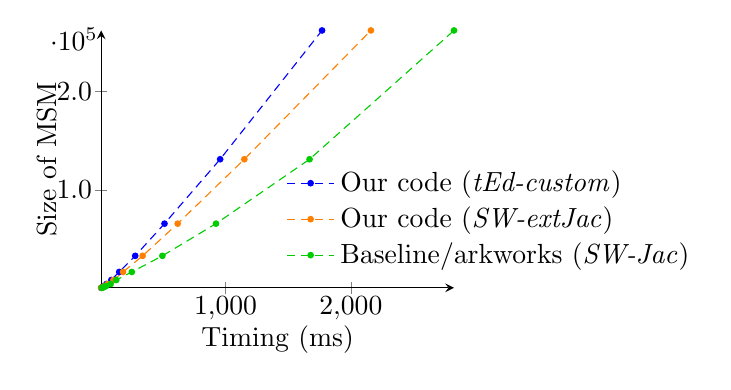
\begin{tikzpicture}
\begin{axis}[
legend style={at={(0.5,0.5)}, anchor=north west, cells={anchor=west}, draw=none, fill=none},
grid=none,
width=0.5\textwidth,
height=0.4\textwidth,
axis y line=left,
every axis y label/.style={at={(-0.1,0.5)},anchor=south,rotate=90},
every axis x label/.style={at={(0.5,0.0)},yshift=-10pt,anchor=north},
every x tick label/.style={at={(0,0)},anchor=north,inner sep=1pt},
every y tick label/.style={at={(0,0)},anchor=east,inner sep=1pt,/pgf/number format/fixed,/pgf/number format/fixed zerofill,/pgf/number format/precision=1,},
every x tick scale label/.style={at={(1,0)},xshift=1pt,yshift=-2pt,anchor=north east,inner sep=0pt},
every y tick scale label/.style={at={(0,1)},xshift=-1pt,yshift=1pt,anchor=north east,inner sep=0pt},
axis x line=bottom,
xlabel = {Timing (ms)},
ylabel = {Size of MSM},
]
\pgfplotstableread[row sep=\\]{
       y log2y   our-tEd   our-sw     arkworks \\
     256   8       7.66     7.63      12.76   \\
     512   9      10.46     13.52     19.44   \\
    1024  10      17.23     20.25     29.97   \\
    2048  11      29.90     35.97     47.38  \\
    4096  12      49.16     58.93     83.38   \\
    8192  13      88.55     105.58    127.92  \\
   16384  14     151.28     182.52    252.21  \\
   32768  15     279.15     338.3     496.06  \\
   65536  16     512.91     617.99    923.79  \\
  131072  17     956.89     1150.00   1670.49 \\
  262144  18    1770.00    2160.00    2823.12\\
}\dataGMSM
\addplot [mark=*, densely dashed, mark size=1pt, \MBlue, mark options={solid,fill=\MBlue, draw=\MBlue}]
table[x index=2,y index=0, header=true]{\dataGMSM} ;
\addlegendentry[align=left]{Our code (\textit{tEd-custom})}
\addplot [mark=*, densely dashed, mark size=1pt, \MOrange, mark options={solid,fill=\MOrange, draw=\MOrange}]
table[x index=3,y index=0, header=true]{\dataGMSM} ;
\addlegendentry[align=left]{Our code (\textit{SW-extJac})}
\addplot [mark=*, densely dashed, mark size=1pt, \MGreen, mark options={solid,fill=\MGreen, draw=\MGreen}]
table[x index=4,y index=0, header=true]{\dataGMSM} ;
\addlegendentry[align=left]{Baseline/arkworks (\textit{SW-Jac})}
\end{axis}
\end{tikzpicture}
\end{scriptsize}
\end{sffamily}
\end{figure}

For the ZPrize MSM instance of size $2^{16}$ the speed up is 45\% with the
\textit{tEd} version and 33\% with the more generic \textit{SW-extJac}
version. For different sizes ranging from $2^8$ to $2^{18}$ the speed up
is 40-47\% with the \textit{tEd} version and 20-35\% with \textit{SW-extJac}.

\section{Conclusion}
Multi-scalar-multiplication dominates the proving cost in most
elliptic-curve-based SNARKs.  Inner curves such as the BLS12-377 are optimized
elliptic curves suitable for both proving generic-purpose statements and in
particular for proving composition and recursive statements.  Hence, it is
critical to aggressively optimize the computation of MSM instances on these
curves.  We showed that our work yield a very fast implementation both when the
points are given on a short Weierstrass curve and even more when the points are
given on a twisted Edwards curve. We showed that this is always the case for
inner curves such as BLS12-377 and that the conversion cost is a one-time
computation that can be performed in the \textit{Setup} phase. We note that,
more generally, these tricks apply to any elliptic curve that admits a twisted
Edwards form — particularly SNARK-friendly 2-cycles of elliptic curves. We
suggest that this should be taken into account at the design level of
SNARK-friendly curves.

\textit{Open-question:} For the Groth16 SNARK~\cite{EC:Groth16}, the same
scalars $a_i$ are used for two MSMs on two different elliptic curves ($\G_1$
and $\G_2$ MSMs where these and the pairing groups).  We ask if it is possible
to mutualize a maximum of computations between these two instances? It seems
that moving to a type-2 pairing would allow to deduce the $\G_1$ instance from
the $\G_2$ one using an efficient homomorphism over the resulting single point.
However, $\G_2$ computations would be done on the much slower full extension
$\F_{p^k}$ (instead of $\F_{p^{k/d}}$ where $d$ is the twist degree).  The
pairing, needed for proof verification, would also be slower.

\section*{Acknowledgement}
The two co-authors of this paper are also co-authors of the
\texttt{gnark-crypto} library. We thank the other co-authors Thomas Piellard,
Ivo Kubjas, Arya Pourtaba Tabaie and Gus Gutoski for their contributions to
\texttt{gnark-crypto}, which allowed this work. We also acknowledge that the
appendix of this paper is a reprint of the material as it appears in a blog
note we shared in 2020 on \url{hackmd.io}. This note was never published in an
academic paper.
% \newpage
\appendix
\section{Faster \texttt{bigint} modular multiplication for most moduli}
\label{appendix}
We discovered an optimization that reduces the number of operations needed to
compute the modular multiplication of two big integers for most (but not quite
all) choices of modulus. To the best of our knowledge, we are not aware of any
prior art describing this optimization, though it is possible that we missed
something in the literature.
%
\subsection{The Montgomery multiplication: theory}
\paragraph{The modular multiplication problem.}
Given integers $a$, $b$ and $p$ the modular multiplication problem is to
compute the remainder of the product
$$ ab \mod p~.$$

On computers a division operation is much slower than other operations such as
multiplication. Thus, a naive implementation of $ab \mod p$ using a
division operation is prohibitively slow.  In 1985, Montgomery introduced a
method to avoid costly divisions~\cite{Montgomery85}. This method, now called the Montgomery
multiplication, is among the fastest solutions to the problem and it continues
to enjoy widespread use in modern cryptography.

\paragraph{Overview of the solution: the Montgomery multiplication.}
There are many good expositions of the Montgomery multiplication
(e.g.~\cite{EPRINT:BosMon17}). As such, we do not go into detail on the
mathematics of the Montgomery multiplication. Instead, this section is intended
to establish notation that is used throughout this appendix.

The Montgomery multiplication algorithm does not directly compute $ab \mod p$.
Instead it computes $abR^{-1} \mod p$ for some carefully chosen number $R$
called the Montgomery radix. Typically, $R$ is set to the smallest power of two
exceeding $p$ that falls on a computer word boundary. For example, if $p$ is
381 bits then $R = 2^{6\times 64} = 2^{384}$ on a 64-bit architecture.

In order to make use of the Montgomery multiplication the numbers $a$ and $b$
must be encoded into the Montgomery form: instead of storing $(a,b)$, we store
the numbers $(\tilde{a}, \tilde{b})$ given by $\tilde{a}=aR \mod p$ and
$\tilde{b}=bR \mod p$.  A simple calculation shows that the Montgomery
multiplication produces the product $ab \mod p$, encoded in the Montgomery
form: $(aR)(bR)R^{-1}=abR \mod p$.  The idea is that numbers are always stored
in the Montgomery form so as to avoid costly conversions to and from the
Montgomery form.

Other arithmetic operations such as addition, subtraction are unaffected by the
Montgomery form encoding. But the modular inverse computation $a^{-1} \mod p$
must be adapted to account for the Montgomery form. We do not discuss modular
inversion in this appendix.

\subsection{The Montgomery multiplication: implementation}
For security purposes, cryptographic protocols use large moduli — $a$ ,$b$ and
$p$ are stored on multiple machine words (multi-precision). In this appendix,
we let $D$ denote the basis in which integers are represented. (For example,
$D=2^{64}$ if a word is 64 bits). A large number $n$ can be represented by its
base-$D$ digits $n_0, \dots, n_m$ stored in machine words (\texttt{uint}):
$\sum_{i=0}^m n_i D^i$.

There are several variations of multi-precision Montgomery multiplication. A
popular choice is the Coarsely Integrated Operand Scanning (CIOS)
variant~\cite{acar1998high-speed}.  In some settings, factors such as modulus
size, CPU cache management, optimization techniques, architecture and available
instruction set might favor other variants.

\paragraph{How fast is the CIOS method?}
Let $N$ denote the number of machine words needed to store the modulus $p$.
For example, if $p$ is a 381-bit prime and the hardware has 64-bit word size
then $N=6$.  The CIOS method solves modular multiplication using $4N^2+4N+2$
unsigned integer additions and $2N^2+N$ unsigned integer multiplications.

Our optimization reduces the number of additions needed in the CIOS Montgomery
multiplication to only $4N^2-N$, a saving of $5N+2$ additions.  This
optimization can be used whenever the highest bit of the modulus is zero (and
not all of the remaining bits are set — see below for details).

The core of the state-of-the-art CIOS Montgomery multiplication is reproduced
below. This listing is adapted from Section 2.3.2 of Tolga Acar’s
thesis~\cite{acar1998high-speed}. The symbols in this listing have the
following meanings:

\begin{itemize}
    \item $N$ is the number of machine words needed to store the modulus $p$.
    \item $D$ is the word size. For example, on a 64-bit architecture $D$ is $2^{64}$.
    \item $a[i], b[i], p[i]$ are the $i$-th words of the integers $a$, $b$ and $p$.
    \item $p'[0]$ is the lowest word of the number $-p^{-1} \mod R$. This quantity is precomputed, as it does not depend on the inputs  $a$ and $b$.
    \item $t$ is a temporary array of size $N+2$.
    \item $C$, $S$ are machine words. A pair $(C,S)$ refers to (high-bits, low-bits) of a two-word number. For short we denote them $(\texttt{hi}, \texttt{lo})$.
\end{itemize}
%
\begin{algorithm}[hbt]
    \SetAlgoLined
    \For{$i=0$ to $N-1$}{
        $C := 0$\;
        \For{$j=0$ to $N-1$}{
            $(C,t[j]) := t[j] + a[j]\cdot b[i] + C$
        }
        $(t[N+1],t[N]) := t[N] + C$\;
        $C := 0$\;
        $m := t[0]\cdot p'[0] \mod D$\;
        $(C,\_) := t[0] + m \cdot p[0]$\;
        \For{$j=1$ to $N-1$}{
            $(C,t[j-1]) := t[j] + m \cdot p[j] + C$
        }
        $(C,t[N-1]) := t[N] + C$\;
        $t[N] := t[N+1] + C$\;
    }
  \caption{The CIOS Montgomery multiplication}
  \label{alg:cios-mont-mul}
\end{algorithm}

Next, we show that we can save the additions in lines 5 and 12 of
Alg.~\ref{alg:cios-mont-mul} when the highest word of the modulus $p$ is at
most $(D-1)/2-1$. This condition holds if and only if the highest bit of the
modulus is zero and not all of the remaining bits are set.

\paragraph{Our optimization.}
Observe that lines 4 and 10 have the form $(\texttt{hi}, \texttt{lo}) :=
m_1+m_2\cdot B+m_3$, where $\texttt{hi}$, $\texttt{lo}$, $m_1$, $m_2$, $m_3$
and $B$ are machine-words where each is at most $D-1$. If $B \leq (D-1)/2-1$
then a simple calculation shows that
%
\begin{align*}
    m_1+m_2\cdot B+m_3 &\leq (D-1)+(D+1)(\tfrac{D-1}{2}-1)+(D-1) \\
                       &\leq D\underbrace{(\tfrac{D-1}{2})}_\texttt{hi}+\underbrace{(\tfrac{D+1}{2}-1)}_\texttt{lo}
\end{align*}
%
From which we derive the following Lemma:
%
\begin{lemma}
    \label{fact1}
    If $B \leq (D-1)/2-1$, then $\texttt{hi} \leq (D-1)/2$.
\end{lemma}
%
We use Lemma~\ref{fact1} to prove the following Proposition:
%
\begin{proposition}
    \label{fact2}
    If the highest word of $p$ is at most $(D-1)/2-1$, then the variables
    $t[N]$ and $t[N+1]$ always store the value 0 at the beginning of each
    iteration of the outer $i$-loop.
\end{proposition}
%
\begin{proof}
    We prove this proposition by induction.  The base case $i=0$ is trivial,
    since the $t$ array is initialized to 0.  For the inductive step at the
    iteration $i$, we suppose that $t[N]=t[N+1]=0$ and trace the execution
    through the iteration.  Begin at the final iteration of the first inner
    loop ($j=N-1$) on line 4. Because $a<p$ and because the highest word of $p$
    is smaller than $(D-1)/2$, we may use Lemma~\ref{fact1} to see that the
    carry $C$ is at most $(D-1)/2$.  Then line 5 sets
    \begin{align*}
    t[N] &= C \\
    t[N+1] &= 0~.
    \end{align*}
    A similar observation holds at the end of the second inner loop ($j=N-1$)
    on line 10: Lemma~\ref{fact1} implies that the carry $C$ is at most
    $(D-1)/2$.  We previously observed that $t[N]$ is also at most $(D-1)/2$,
    so $t[N] + C$ is at most
    $$ \tfrac{D-1}{2} + \tfrac{D-1}{2} = D-1$$
    which fits entirely into a single word. Then line 11 sets $C$ to 0 and line
    12 sets $t[N]$ to 0.  The proof by induction is now complete.
\end{proof}

With this proposition, we no longer need the addition at line 5. We store $C$
in a variable $A$ and at line 11 we compute instead
$$ (\_,t[N-1]) := A + C $$

\paragraph{The final algorithm.} For $N < 12$, we merge the two inner loops
%
\begin{algorithm}[hbt]
    \SetAlgoLined
    \For{$i=0$ to $N-1$}{
        $(A,t[0]) := t[0] + a[0]\cdot b[i]$\;
        $m := t[0]\cdot p'[0] \mod W$\;
        $C,_ := t[0] + m\cdot p[0]$\;

        \For{$j=1$ to $N-1$}{
            $(A,t[j])  := t[j] + a[j]\cdot b[i] + A$\;
            $(C,t[j-1]) := t[j] + m\cdot p[j] + C$\;
        }
        $t[N-1] := C + A$\;
    }
  \caption{Our optimized CIOS Montgomery multiplication}
  \label{alg:opt-cios-mont-mul}
\end{algorithm}

\paragraph{Our optimized Montgomery squaring.}
The condition on the modulus differs, here
$$ p[N-1] \leq \tfrac{D-1}{4} - 1~.$$
However, the reasoning is similar and we end up with
%
\begin{algorithm}[hbt]
    \SetAlgoLined
    \For{$i=0$ to $N-1$}{
        $C, t[i] := a[i] \cdot a[i] + t[i]$\;
        $p := 0$\;
        \For{$j=i+1$ to $N-1$}{
            $p,C,t[j] := 2a[j]\cdot a[i] + t[j] + (p,C)$
        }
        $A := C$\;
        $m := t[0] \cdot p'[0]$;
        $C, _ := t[0] + p[0]\cdot m$
        \For{$j=1$ to $N-1$}{
            $C, t[j-1] := p[j]\cdot m +  t[j] + C$
        }
        $t[N-1] := C + A$\;
    }
  \caption{Our optimized CIOS Montgomery squaring}
  \label{alg:opt-cios-mont-sq}
\end{algorithm}

\bibliographystyle{alpha}
\bibliography{refs}

\end{document}
